\documentclass[11pt]{article}
\usepackage{geometry}                % See geometry.pdf to learn the layout options. There are lots.
\geometry{letterpaper}                   % ... or a4paper or a5paper or ... 
\usepackage{graphicx}
\usepackage{amssymb}
\usepackage{epstopdf}
\usepackage{float}

\title{Bag-of-Words based Image Classification}
\author{R\'emi de Zoeten and Anouk Visser}

\begin{document}
\maketitle
\section{Introduction}
In this report we will discuss the implementation and results of a system for image classification. The system can tell if there is an object of one of four given classes (motorbikes, cars, faces and airplanes) in an image. The classification system is based on a Bag-of-Words approach, meaning that the Support Vector Machine that performs the classification uses histograms of words for training and classification of an image. The words are obtained by extracting descriptors from a set of training images and cluster them using the \textit{kmeans} algorithm.  

\section{Implementation}
We have extracted key point SIFT features and dense SIFT features. In addition to this we have also trained and evaluated our system using RGBSIFT, rgbSIFT and opponentSIFT, these are just key point- or dense SIFT features applied to all three of the color channels of the specific colorspace, resulting in descriptors of dimension $(128\times3)\times1$. For dense SIFT sampling we used a bin size of 10 pixels and a step size of 5. \\
To build a visual vocabulary, we use the extracted descriptors from a number of training images (of all classes) and use this as the data for the kmeans clustering algorithm. The number of clusters represents the number of words in the vocabulary. Because of our limited computational resources the largest vocabulary we have built is a vocabulary of $100$ words based on $5$ training images. \\
We will then use the words to quantize training and test images. We do this by extracting descriptors from the image and find the descriptor from the vocabulary with the smallest euclidean distance with respect to the descriptor from the image. We will keep track of which words (i.e. descriptors from the vocabulary) were selected and how many times this happened in a histogram. When every descriptor has been `matched' to a word from the vocabulary, we normalize the resulting histogram by dividing every bin by the total number of descriptors extracted from the image. We perform this quantization on both the images for training and testing. \\
The histograms of the training images are then used to train a Support Vector Machine. We train one SVM for every class, for the `motorbikes' we will use the histograms of training images of a motorbike as positive examples and histograms of the other images as negative examples. After we have trained the classifiers we can use these to make predictions about the test histograms.\\
As an evaluation measure we have used the Mean Average Precision. We provide every classifier with all the test images and rank the results based on the probability that the test image is off the class the classifier is trained on. For every classifier we will thus have a ranked list of test images, if everything works well the top of the list should be dominated by images of the class the classifier can predict. In the next section we will show the results of our system and provide an analysis of these results. 


\section{Evaluation}

\subsection{Size of the training set}
\label{train}
The first experiment we will discuss measures the performance of the system for all different methods of SIFT (dense and key point combined with all colorspaces results in a total of eight methods). We have set out the Mean Average Precision against the number of images that were used to train the SVM. The results of this experiment can be found in figure \ref{trainingSizes}. The first thing that stands out is the rather large difference between the key point SIFT features and the dense SIFT features. It appears that dense SIFT features perform much better than key point SIFT features. Performance of all methods increases rapidly up until using approximately 40 training images. However, after this point there is only a slight increase in performance when increasing the training size. Only key point SIFT applied to the rgb colorspace shows a sudden peak in performance, we are not sure whether this is actually happening or that we can consider this as noise in the data. 
\begin{figure}[H]
  \centering
    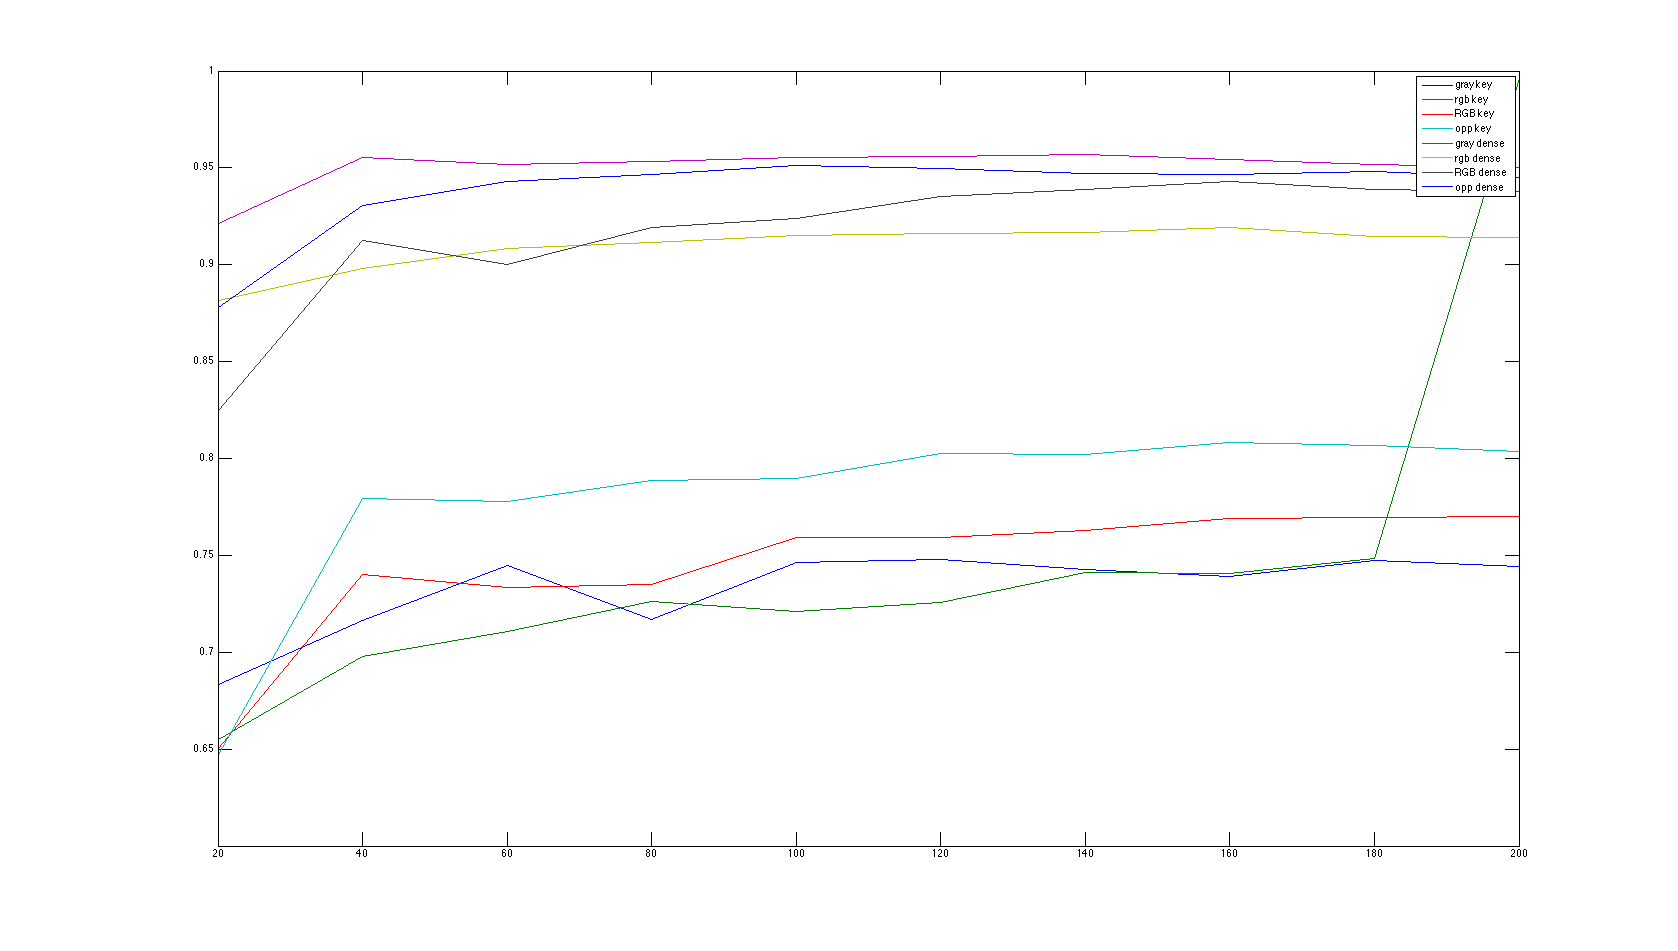
\includegraphics[width=0.75\textwidth]{trainingSizes}
      \caption{Results of the system for different sizes of the set of image histograms used to train the SVM. The SVM was trained using an RBF kernel. For this experiment we have used a vocabulary size of 50 that was made by clustering the descriptors of 10 images from each training class.}
      \label{trainingSizes}
\end{figure}

\subsection{Size of the vocabulary}
Similar to the experiment described in section \ref{train} we have performed an experiment in which we measured performance for all different methods under varying vocabulary sizes, the results of which are shown in figure \ref{vocabularySizes}. Again we find that the dense SIFT features perform better than the key point SIFT features, with the exception of the key point SIFT applied to the rgb color space. The rgb color space shows excellent performance for all different vocabulary sizes. We are unsure why this is the case, but after careful inspection of the classifiers trained on these features we have concluded that it really performs this well and that it is not just noise. We observe that the majority methods benefit from a larger vocabulary size. 
\begin{figure}[H]
  \centering
    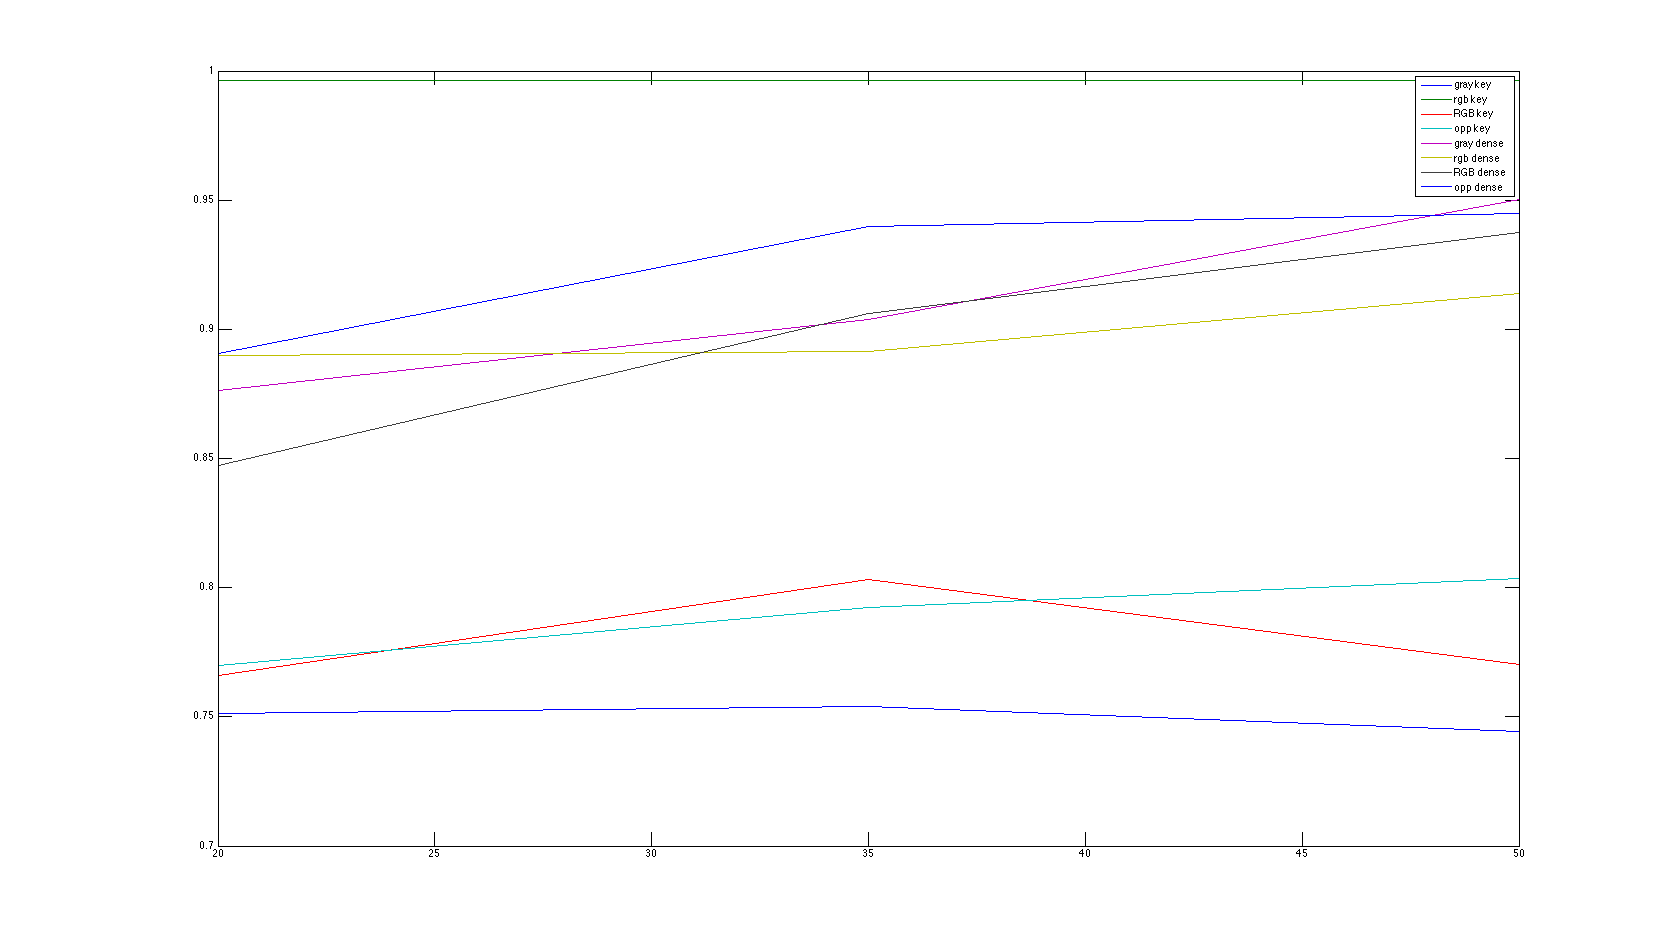
\includegraphics[width=0.75\textwidth]{vocabularySizes}
      \caption{Results of the system for different sizes of the vocabulary. For this experiment we used the descriptors of 10 images from each training class to build the vocabulary. We used 200 image histograms from each class to train the SVM. The SVM was trained using an RBF kernel.}
      \label{vocabularySizes}
\end{figure}

\subsection{Kernel functions for the SVM}
Finally, we performed experiments in which we varied the kernel used for training the SVM. Figure \ref{kernels} shows the result for different kernels on both dense and key point SIFT in the grey colorspace. It is clear that the polynomial kernel is not a good choice to solve this problem. The linear kernel outperforms the rest, although it is really similar to both the polynomial kernel and the sigmoid kernel.  
\begin{figure}[H]
  \centering
    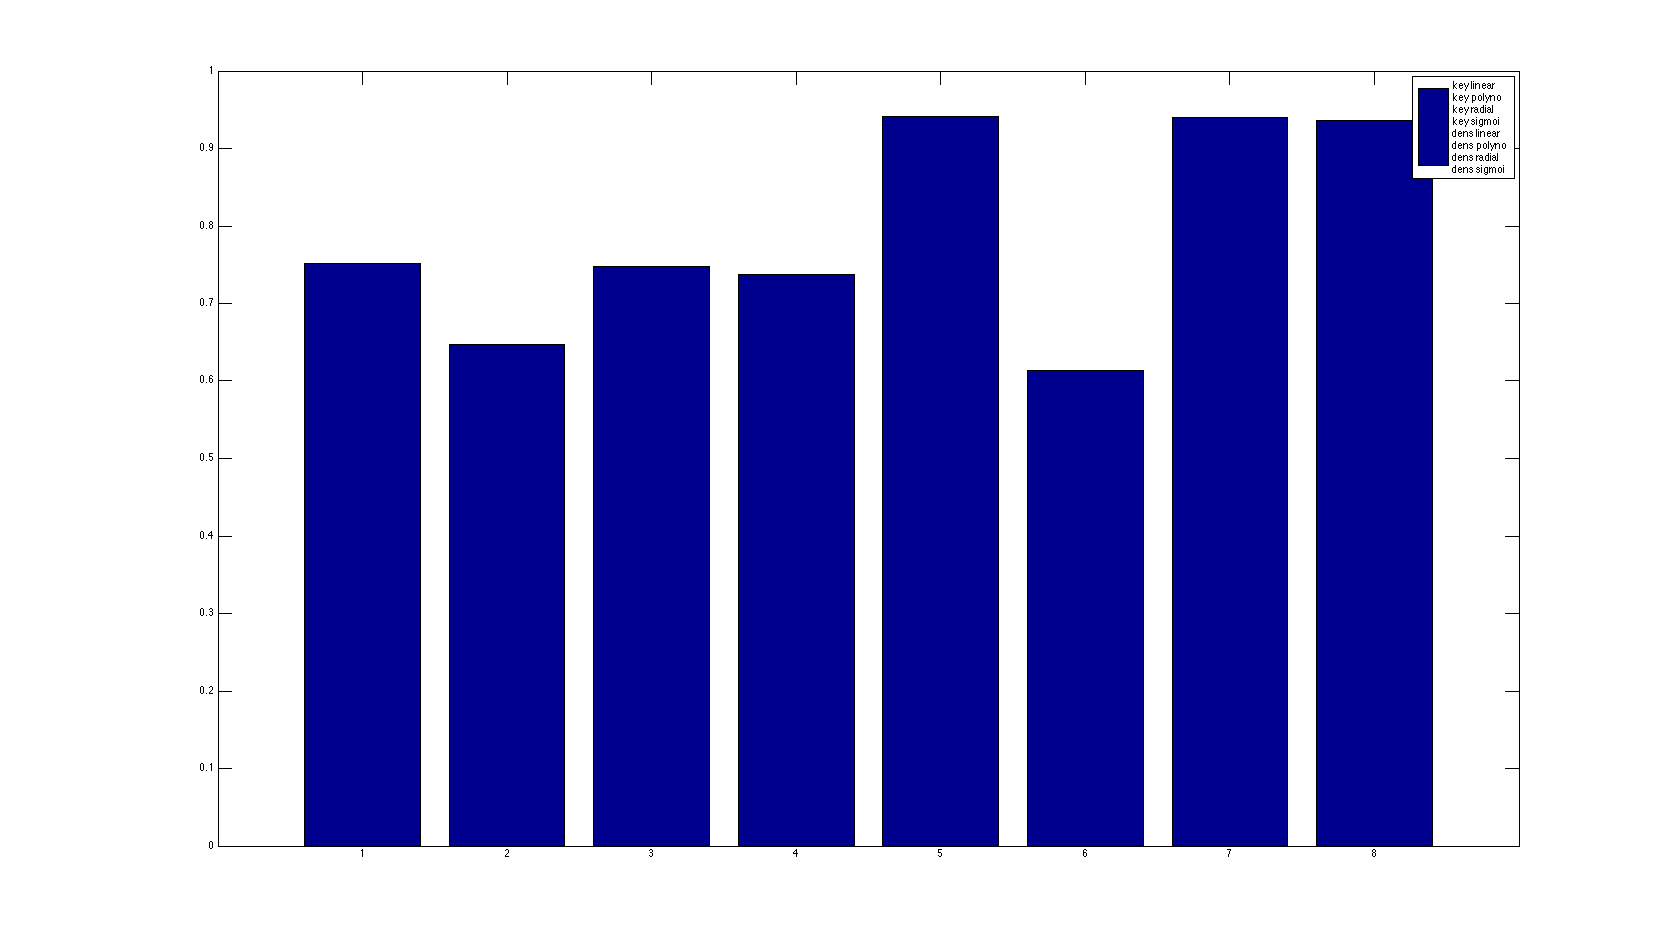
\includegraphics[width=0.75\textwidth]{greyKernels}
      \caption{Results of the system for different kernels used for training the SVM. For this experiment we have used a vocabulary size of 100 that was made by clustering the descriptors of 5 images from each training class. We used 200 image histograms from each class to train the SVM. From left to right this figure shows the MAP for key point SIFT grey: linear, polynomial, RBF and sigmoid kernel, followed by the dense point SIFT grey: linear, polynomial, RBG and sigmoid kernel. }
      \label{kernels}
\end{figure}

\section{Conclusion}
In this report we have discussed our implementation of a system for image classification based on a Bag-of-Words approach. We have shown its performance for different sizes of the training data, different vocabulary sizes, different SIFT features for different colorspaces and different kernels used to train the SVM. Unfortunately we did not have the computing power to perform any larger tests (for instance larger vocabularies based on larger training sets). However, we found that the results using smaller vocabulary sizes were above expectations. 
%Please, make a simple document with four ranked lists of test images as discussed in Section 2.6. This document should also contain all your settings (size of visual vocabulary, number of positive and negative samples, and so on), Average Precision per class, and Mean Average Precision.


\end{document}  